\documentclass[11pt,a4paper]{report}
\usepackage[utf8]{inputenc}
\usepackage[french]{babel}
\usepackage[T1]{fontenc}
\usepackage{amsmath}
\usepackage{amsfonts}
\usepackage{amssymb}
\usepackage{xcolor}

\usepackage{geometry}
\geometry{hmargin=2.5cm,vmargin=1.5cm}
\usepackage{wasysym}
\usepackage{graphicx}

\author{Mathieu Sarrat}
\title{LP17 - Interférences à deux ondes en optique}

\makeatletter
\renewcommand{\thesection}{\@arabic\c@section}
\makeatother


\begin{document}
\maketitle

\section*{Pré-requis}
\begin{itemize}
	\item Chemin optique, lentilles minces, miroirs plans
	\item Modèle scalaire de la lumière
	\item Transformation de Fourier
\end{itemize}

\newpage
\section*{Introduction}

Soit une source de lumière et un détecteur. Un détecteur de lumière est sensible à la puissance lumineuse qu'il reçoit. Nous avons vu lors d'une leçon précédente que la lumière pouvait être décrite comme une onde électromagnétique, c'est à dire par un champ électromagnétique se propageant dans l'espace en transportant de l'énergie. La quantité clé de ce transport est donnée par le vecteur de Poynting $\bold{R}$, qui traduit un flux d'énergie électromagnétique par unité de surface. Son module s'exprime en $\text{W}.\text{m}^{-2}$ ce qui en fait une puissance surfacique.\\

La durée caractéristique d'une onde électromagnétique visible est donnée par l'inverse d'une fréquence typique de ces ondes $f_h$. L'œil possède une sensibilité maximale pour $\lambda_h \simeq 550 \text{nm}$, d'où $f_h = c/\lambda_h = 5\times10^{14}$ Hz, d'où une durée typique
\begin{equation}
	\boxed{\tau_h \simeq 10^{-15}\text{s}}.\\
\end{equation}

Lorsqu'un signal atteint un détecteur, on doit se poser la question du temps de réponse du détecteur. Notre œil ou tout autre détecteur de lumière n'échappe pas à cette nécessité :

\begin{center}
\begin{tabular}{|c|c|}
  \hline
  	\textbf{Détecteur} & \textbf{Temps de réponse} $\tau_r$ en s\\
  \hline
  \hline
  	Oeil & $10^{-1}$\\
  \hline 
  	Capteur CCD & $10^{-2}$\\
  \hline
  	Pellicule photo & $10^{-4}$ à $10^{-5}$\\
  \hline
   	Photodiode & $10^{-6}$ à $10^{-9}$\\
  \hline
\end{tabular}
\end{center}

Quelque soit le détecteur à notre disposition, on a
\begin{equation}
	\boxed{\tau_r \gg \tau_h}.
\end{equation}

En pratique, un détecteur de lumière sera sensible \textbf{à la puissance moyenne} qu'il reçoit du champ électromagnétique. On définit \textbf{l'éclairement} (puisque c'est ce qu'on voit) au point $M$ d'observation comme la valeur moyenne du module du vecteur de Poynting en ce point :
\begin{equation}
	\boxed{\mathcal{E}(M) = \left\langle ||\bold{R}(M)|| \right\rangle _t
	= \epsilon_0 c \left\langle E^2(M) \right\rangle_t}. 
\end{equation} 
C'est en cela qu'on dit que les détecteurs en optique sont quadratiques : ils sont sensibles au carré du champ électrique.\\

En pratique, il n'y a jamais qu'une seule source de lumière : étoiles dans le ciel, lampes dans une salle de classe, feux de signalisation et phares des voitures la nuit en ville. Que se passe-t-il lorsque deux sources de lumière sont présentes et cela a-t-il un impact sur l'éclairement que nous observons ? Faisons une expérience. \textcolor{red}{Manip qualitative d'introduction (voir en Annexe)}.\\ 

Pourtant lorsqu'on allume deux lampes dans une pièce sombre, on ne voit pas ces alternances de zones lumineuses et de zones obscures. Ce phénomène est un phénomène d'interférences. L'objectif de cette leçon va être dans un premier temps d'expliquer cette répartition surprenante de la lumière que nous venons de constater, puis de comprendre pourquoi on ne voit pas ces "franges" partout, toute la journée, compte tenu de la multitude de sources de lumière qui nous entourent !

\newpage
\section{Superposition de deux ondes lumineuses}

Les équations de Maxwell qui décrivent le comportement d'un champ électromagnétique sont linéaires : toute combinaison linéaire de solutions est elle-même solution des équations. Nous avons vu que toute onde progressive pouvait s'écrire comme une superposition d'ondes progressives monochromatiques/harmoniques (OPPM).\\

Une source ponctuelle va émettre des ondes sphériques, par symétrie. Si on place le détecteur suffisamment loin des sources, les ondes qu'il recevra pourront être approximées correctement par des ondes planes. Nous allons donc considérer deux sources ponctuelles monochromatiques émettant des OPPM.

\subsection{Conditions d'interférences}

Soient
\begin{equation}
	\bold{E}_1(M,t) = \bold{E}_{01}\;\text{cos}(\omega_1 t - \phi_1(M)),
\end{equation}
émise par la source 1, où $\phi_1(M)$ désigne la phase de l'onde au point M par rapport à l'origine des temps, et
\begin{equation}
	\bold{E}_2(M,t) = \bold{E}_{02}\;\text{cos}(\omega_2 t - \phi_2(M)),
\end{equation}
onde émise par la source 2.\\

\textbf{Remarque :} ondes planes progressives monochromatiques, donc la phase à l'origine ne dépend pas du temps. Ce ne sera plus le cas lorsqu'on considèrera des trains d'ondes dans la partie Cohérences.\\

Par linéarité des équations de Maxwell, l'onde lumineuse au point M a pour champ électrique
\begin{equation}
	\boxed{\bold{E} = \bold{E}_1 + \bold{E}_2},
\end{equation}
et l'éclairement au point M est donné par
\begin{equation}
	\mathcal{E}(M) = \epsilon_0 c \left\langle (\bold{E}_1 + \bold{E}_2)^2 \right\rangle
\end{equation}
d'où
\begin{equation}
	\mathcal{E}(M) = \frac{1}{2}\epsilon_0 c E_{01}^2 + \frac{1}{2}\epsilon_0 c E_{02}^2
	+ \epsilon_0 c \bold{E}_{01}\cdot\bold{E}_{02}
	\left[
	\left\langle \text{cos}\left[(\omega_1 + \omega_2)t - (\phi_1 + \phi_2) \right]\right\rangle 	  + \left\langle \text{cos}\left[(\omega_1 - \omega_2)t - (\phi_1 - \phi_2) \right]\right\rangle
	\right]
\end{equation}

Le terme en cos$(\omega_1 + \omega_2)t$ est \textbf{toujours nul}, d'où
\begin{equation}
	\mathcal{E}(M) = \mathcal{E}_1 + \mathcal{E}_2 
	+ \epsilon_0 c \bold{E}_{01}\cdot\bold{E}_{02} 
	\left\langle \text{cos}\left[(\omega_1-\omega_2)t+(\phi_2-\phi_1)\right]\right\rangle
\end{equation}

De façon générale, l'éclairement total n'est pas égal à la somme des éclairements liés à chacune des deux sources. Il existe un troisième terme, qu'on appelle \textbf{terme d'interférences}.\\

On dit qu'il y a interférences lorsque ce troisième terme n'est pas nul, c'est à dire lorsque les deux ondes sont \textbf{cohérentes} : l'éclairement résultant de la superposition de deux sources n'est pas égal à la somme des éclairements de chaque source. Introduisons donc \textbf{deux conditions de cohérence} pour observer des interférences \textbf{\textcolor{red}{avec des OPPM}} :
\begin{itemize}
	\item $\omega_1 = \omega_2$ : les OPPM doivent avoir la même fréquence; 
	\item $\bold{E}_{01}\cdot\bold{E}_{02} \neq 0$ : les OPPM ne doivent pas avoir des 						polarisations orthogonales.\\
\end{itemize}

Dans ce cas,
\begin{equation}
	\boxed{\mathcal{E} = 
	\mathcal{E}_1 + \mathcal{E}_2 
	+ \epsilon_0 c \;\bold{E}_{01}\cdot\bold{E}_{02}\;\text{cos}\left(\phi_2-\phi_1\right)}
\end{equation}
\textbf{Remarque 1 :} deux ondes de fréquences différentes n'interfèreront pas et l'éclairement lié à la superposition de ces deux ondes sera égal à la somme des éclairements.\\
\textbf{Remarque 2 :} loin des sources, les directions de propagation sont voisines et on peut adopter un modèle scalaire de la lumière (Sanz p736), ce que nous ferons par la suite.\\

\subsection{Interférences}

On considère désormais des vibrations scalaires observées loin des sources en supposant les conditions de cohérence précédentes assurées (cohérence totale) :
\begin{equation}
	s_i(M,t) = s_{0,i} \text{cos}\left(\omega t - \phi_{i}(M) \right),
	\label{eq:11}
\end{equation}
et l'éclairement résultant de la superposition\footnote{le 2 provient du fait qu'on suppose une lumière non-polarisée : les composantes $E_x$ et $E_y$ du champ total sont statistiquement équivalentes} 
\begin{equation}
	\mathcal{E}(M) = 2\left\langle (s_1(M,t) + s_2(M,t))^2\right\rangle 
	= s_{0,1}^2 + s_{0,2}^2 + 2 s_{0,1} s_{0,2} \text{cos}\left(\phi_2-\phi_1\right)
	\label{eq:12}
\end{equation}
en injectant \eqref{eq:11} dans \eqref{eq:12} et en utilisant les propriétés de la moyenne temporelle. Si on introduit l'éclairement propre à chaque source, on obtient la \textbf{formule de Fresnel :}
\begin{equation}
	\boxed{\mathcal{E}(M) = \mathcal{E}_1(M) + \mathcal{E}_2(M) 
	+ 2\sqrt{\mathcal{E}_1(M)\mathcal{E}_2(M)}\; \text{cos}\left(\Delta \phi (M)\right)}.
\end{equation}

Pour simplifier, on peut supposer $\mathcal{E}_1(M) = \mathcal{E}_2(M) = \mathcal{E}_0(M)$, d'où
\begin{equation}
	\boxed{\mathcal{E}(M) = 2\mathcal{E}_0(M)\left[1 
	+ \text{cos}\;\left(\Delta\phi(M)\right)\right]}.\\
\end{equation}
 
Il ne reste plus qu'à exprimer la différence de phase au point M entre les deux ondes $\Delta\phi(M)$. Dans le cas présent, deux sources ponctuelles d'OPPM, cette différence de phase est constante dans le temps et peut s'exprimer directement en fonction de la différence de chemin optique (également appelée différence de marche) $\delta(M)$ parcouru par les deux ondes :
\begin{equation}
	\boxed{\Delta \phi (M) = \frac{2\pi}{\lambda_0}\delta(M)} \quad\text{avec}\quad
	\delta(M) + \Delta\varphi,
\end{equation}
avec
\begin{equation}
	\delta(M) = L\left(S_2M\right) - L\left(S_1M\right) \quad\text{et}\quad	L(S_i M) 
	= \int_{S_i}^M nds
\end{equation}
et $\Delta\varphi = \varphi(S_2) - \varphi(S_1)$ la différence de phase à l'origine des temps et de l'espace, constante dans le cas des deux OPPM. On supposera, par souci de simplicité, que les sources sont en phase, d'où $\Delta\varphi = 0$.\\

Finalement, on définit l'\textbf{ordre d'interférences} :
\begin{equation}
	p(M) \equiv \frac{\Delta \phi(M)}{2\pi} = \frac{\delta(M)}{\lambda_0}.\\
\end{equation}

\textcolor{red}{Traçons le profil de l'éclairement en fonction de $\Delta\phi(M)$ (Sanz p738) :}\\

Selon le signe de $\Delta \Phi(M)$, l'éclairement résultant est supérieur ou inférieur à la somme des éclairements de chaque onde :
\begin{itemize}
	\item interférences \textbf{constructives} (franges brillantes) si 
	$\mathcal{E}(M)>\mathcal{E}_1(M)+\mathcal{E}_2(M)$, et \textbf{totalement constructives si $p$ 
	est entier} et donc $\delta$ multiple entier de la longueur d'onde (les deux ondes sont en phase);
	\item interférences \textbf{destructives} (franges sombres) si $\mathcal{E}(M)<\mathcal{E}_1(M)+		\mathcal{E}_2(M)$, et \textbf{totalement destructives si $p$ demi-entier}, les deux ondes étant 		dans ce cas en \textbf{opposition de phase}.\\
\end{itemize}

\textbf{Remarque importante :} le phénomène d'interférences ne crée pas ou ne détruit pas de l'énergie, il ne fait que modifier sa distribution dans l'espace.\\

Définissons le \textbf{contraste},
\begin{equation}
	C \equiv \frac{\mathcal{E}_\text{max} - \mathcal{E}_\text{min}}
	{\mathcal{E}_\text{max} + \mathcal{E}_\text{min}}
\end{equation}
maximal lorsque $\mathcal{E}_1 = \mathcal{E}_2$. La formule de Fresnel se réécrit
\begin{equation}
	\boxed{\mathcal{E}(M) = \mathcal{E}_\text{moy}(M)\left[1 
	+ C\text{cos}\;\left(\Delta\phi(M)\right)\right]} \quad\text{avec}\quad 
	\mathcal{E}_\text{moy} = \frac{\mathcal{E}_1 + \mathcal{E}_2}{2}.
\end{equation}

\subsection{Figure d'interférences}

Indépendamment de la réalisation pratique du système produisant les interférences à deux ondes, du point de vue de l'écran sur lequel on observe le phénomène, les ondes semblent provenir de deux sources. On appelle \textbf{champ d'interférences} la zone de l'espace éclairée simultanément par les deux sources. Le phénomène d'interférences s'observe dans cette région. En plaçant un écran dans le champ d'interférences, on observe une \textbf{figure d'interférences}.\\ 

Cherchons les \textbf{surfaces d'égal éclairement}, telles que $\Delta \phi(M)$ soit constant d'après la formule de Fresnel \textcolor{red}{(Schéma)} :
\begin{equation}
	\Delta \phi(M) = \phi_2(M) - \phi_1(M) = k\left(r_2 - r_1 \right) 
	= \text{cte}
\end{equation}
avec $r_2 = S_2M$ et $r_1 = S_1M$. On reconnaît l'équation d'un \textbf{hyperboloïde de révolution} de foyers $S_1$ et $S_2$.

\subsubsection{Observation dans un plan perpendiculaire au plan médiateur des sources :}

Les franges d'égal éclairement sont des hyperboles. A proximité de l'intersection avec le plan médiateur des sources, ces hyperboles ont une grande excentricité, d'où le fait que ces franges soient \textbf{quasi-rectilignes}.\\

\textbf{Démonstration : \textcolor{red}{Faire un schéma, faire le calcul}}\\

On calcule $\Delta\phi(M) = 2\pi\delta/\lambda_0$ :
\begin{equation}
	\delta = n\left(S_2M - S_1M\right)
\end{equation}
avec
\begin{equation}
	S_2M = \sqrt{\left(x + \frac{a}{2}\right)^2 + y^2 + D^2} 
	= D\sqrt{1 + \frac{y^2}{D^2} + \frac{\left(x+a/2\right)^2}{D^2}}
\end{equation}
et de même
\begin{equation}
	S_1M = D\sqrt{1 + \frac{y^2}{D^2} + \frac{\left(x-a/2\right)^2}{D^2}}.\\
\end{equation}

On observe loin des sources, donc $D \gg a, x, y$, d'où à l'ordre 1 :
\begin{equation}
	\boxed{\delta \simeq n \frac{ax}{D}}\quad\text{d'où}\quad \Delta\phi(M) = 2\pi\frac{ax}{\lambda D}
\end{equation}
et l'éclairement
\begin{equation}
	\boxed{\mathcal{E}(M) = 2\mathcal{E}_0\left[1 + 
	\text{cos}\;\left(2\pi\frac{ax}{\lambda D}\right)\right]}
\end{equation}
ne dépend que de la variable $x$. Le système de franges est invariant par translation le long de $y$, on a bien des franges rectilignes.\\

Deux franges brillantes ($\mathcal{E}(M_i) = \mathcal{E}_(M_{i+1}) = 4\mathcal{E}_0$) sont séparées de
\begin{equation}
	\boxed{i \equiv \frac{\lambda D}{a}}, \quad\textbf{interfrange}.
\end{equation}

Pour $D = 2$m et $\lambda = 0.5 \mu$m, si on veut observer une interfrange $i = 1$mm, il faut deux sources ponctuelles séparées de
\begin{equation}
	a = \frac{\lambda D}{i} = 10^{-3}\text{m} = 1 \text{mm}.
\end{equation}

\subsubsection{Observation dans un plan perpendiculaire à l'axe des sources :}

Le système est invariant par rotation autour de l'axe des sources, aussi lorsque l'écran est perpendiculaire à cet axe, les franges d'égal éclairement prennent la forme d'\textbf{anneaux concentriques}.\\

\textbf{Démonstration : \textcolor{red}{Faire un schéma, parachuter le résultat}}\\
\begin{equation}
	S_2M = \sqrt{x^2 + y^2 + \left(D-a/2\right)^2} = \left(D-\frac{a}{2}\right)\sqrt{1 + \frac{x^2+y^2}{\left(D-a/2\right)^2}} \simeq D-\frac{a}{2} + \frac{x^2+y^2}{2\left(D - a/2\right)}
\end{equation}
loin des sources et
\begin{equation}
	S_1M \simeq D + \frac{a}{2} + \frac{x^2+y^2}{2\left(D + a/2\right)},
\end{equation}
d'où
\begin{equation}
	\boxed{\delta = -na\left(1-\frac{r^2}{2D^2}\right)}
\end{equation}
avec $r^2 = x^2 + y^2$ (coordonnées polaires).\\

D'où l'éclairement au point M
\begin{equation}
	\boxed{\mathcal{E}(M) = 2\mathcal{E}_0 \left[1 
	+ \text{cos}\;\left(2\pi\frac{a}{\lambda}\left(1 - \frac{r^2}{2D^2} \right)\right)\right]},
\end{equation}
de symétrie cylindrique.

\subsubsection{Trous d'Young}

\textcolor{red}{MANIP :} avec un laser focalisable, former un point source le plus fin possible sur les bifentes. On place l'écran d'observation loin des bifentes, pour respecter des conditions de Fraunhöfer approchées $(\lambda D/a^2 >> 1)$. Commenter le phénomène de diffraction qui s'ajoute et qui module la figure d'interférences, mais ne pas s'y attarder, c'est l'objet d'une autre leçon. Bien qu'on n'aie pas rigoureusement des sources ponctuelles, on va appliquer le modèle : on essaye d'interpréter en se ramenant au cas de l'observation dans un plan perpendiculaire au plan médiateur des sources, d'où les franges rectilignes à l'écran. Mesure de l'interfrange en pointant plusieurs zéros successifs puis traitement avec Régressi, résidus etc. En déduire la distance entre le centre des trous et comparer avec une projection effectuée en préparation, pour renforcer la manip (mire, objectif de microscope.\\

\newpage
\section{Cohérence des sources}

La situation permettant d'observer des interférences a jusqu'ici été présentée de manière théorique. Nous sommes partis de deux sources ponctuelles émettant chacune une onde plane progressive monochromatique de pulsations égales, impliquant un retard de phase à l'origine des temps constant entre ces deux ondes.\\ 

Le modèle que nous avons adopté (ondes planes progressives monochromatiques, sources ponctuelles) permet de comprendre l'origine des interférences et de faire des prédictions quantitatives (cf expérience). Il n'est cependant pas complet : l'expérience quotidienne nous montre que deux sources lumineuses indépendantes, comme deux lampes dans une pièce, ne produisent pas d'interférences observables.\\ 

Nous allons donc relâcher une hypothèse. En effet, \textbf{les OPPM n'ont pas de réalité physique :} leur étendue spatiale est illimitée, elles n'ont ni début ni fin dans le temps, impliquant une quantité d'énergie infinie.

\subsection{Modèle des trains d'onde}

Intéressons-nous au fonctionnement des sources lumineuses qui produisent les ondes que nous étudions. L'émission des photons se fait lors de la désexcitation des atomes constituant la source : un électron passe d'un niveau d'énergie supérieur à un niveau inférieur et l'énergie qu'il perd est libérée sous forme de photon d'énergie $E$, associé à une onde électromagnétique de fréquence $\nu$ telle que
\begin{equation}
	E = h\nu,
\end{equation}
$h$ désignant la constante de Planck.\\

L'onde émise de cette manière a nécessairement \textbf{une durée finie}, de l'ordre de $\tau_c \simeq 10^{-11}$s pour une lampe spectrale (vapeur constituée d'un type d'atome, à faible pression). Après l'émission, \textbf{il peut se produire à une date aléatoire} une nouvelle excitation suivie d'une nouvelle désexcitation émettant un photon. Ainsi, plusieurs ondes se succèdent et on dit qu'il y a succession de \textbf{trains d'ondes} \textcolor{red}{(faire un dessin)}. \\

Puisque l'onde lumineuse est émise par trains d'ondes successifs, deux trains en provenance des sources $S_1$ et $S_2$ auront une différence de phase aléatoire. Du point de vue de l'écran, $\Delta\phi(M)$ est une fonction du temps et cette dépendance est aléatoire :
\begin{equation}
	\Delta\phi(M,t) = \varphi(S_2,t) - \varphi(S_1,t) + k\left(S_2M - S_1M\right),
\end{equation}
d'où l'expression de l'éclairement
\begin{equation}
	\mathcal{E}(M) = s_{0,1}^2 + s_{0,2}^2 + 2 s_{0,1} s_{0,2} 
	\underbrace{\left\langle\text{cos}\left(\Delta\phi(M,t)\right) \right\rangle}_{= 0} 
	= s_{0,1}^2 + s_{0,2}^2.
	\label{eq:12}
\end{equation}
Les deux sources sont donc \textbf{incohérentes temporellement} puisqu'elles ne conduisent pas à un phénomène d'interférences.\\

On note $L_c$ l'extension spatiale moyenne d'un train d'ondes, telle que
\begin{equation}
	\boxed{L_c = c\tau_c}.
\end{equation}
Si la différence de chemin optique entre deux trains d'ondes arrivant au point M en provenance de deux sources différentes est inférieure à $L_c$, alors ils vont arriver "l'un sur l'autre" et interférer. Si la différence de marche est supérieure à $L_c$, ils arriveront l'un après l'autre et n'interfèreront pas. Comme $\tau_c$ est petit devant le temps de réponse typique d'un détecteur, la moyenne porte sur un très grand nombre de trains d'onde, qui vont interférer de façon anarchique, ce qui explique l'absence de franges d'interférences dans notre vision quotidienne du monde qui nous entoure.\\

\begin{figure}[h!]
	\begin{center}
		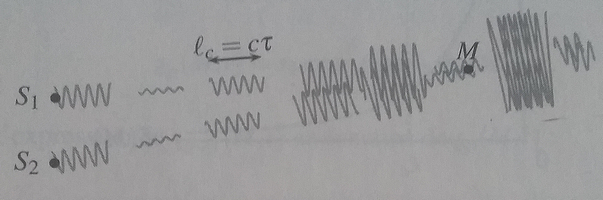
\includegraphics[scale = 0.5]{ordre.png}
	\end{center}
	\caption{Superposition de trains d'ondes si $\delta(M) < L_c$}
\end{figure}

\begin{figure}[h!]
	\begin{center}
		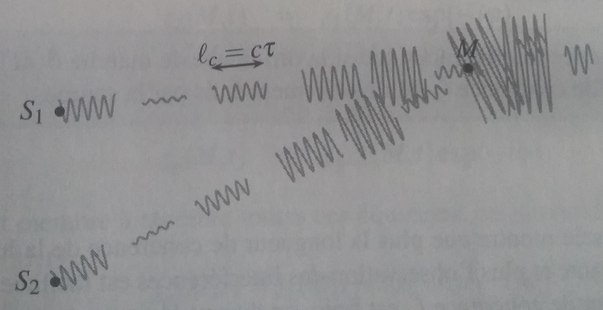
\includegraphics[scale = 0.5]{anarchie.png}
	\end{center}
	\caption{Superposition de trains d'ondes si $\delta(M) > L_c$}
\end{figure}

Une source dont la longueur de cohérence temporelle (et donc la durée de cohérence) est finie présente un \textbf{défaut de cohérence temporelle} et s'éloigne du modèle de l'onde monochromatique.\\

Donnons enfin quelques ordres de grandeur relatifs à plusieurs lampes que l'on utilise en travaux pratiques ou au laboratoire.

\begin{center}
\begin{tabular}{|c|c|c|c|c|c|}
  \hline
  	\textbf{Source}&$\lambda_0$ en nm&$\nu_0$ en $10^{14}$Hz&$\Delta\nu$ en Hz & $\tau_c$ & $\L_c$\\
  \hline
  \hline
  	Lumière blanche & 400 à 800 & 7.5 à 3.5 & $4\times10^{14}$ & $2.5\times10^{-15}$ & 750 nm\\
  \hline 
  	Vapeur de mercure (basse p.) & 546.1 & 5.49 & $10^9$  & $10^{-9}$& 0.3 m\\
  \hline
   	Laser $\text{He}-\text{Ne}$ ordinaire & 632.8 & 4.74 & $10^9$ & $10^{-9}$s & 0.3 m\\
  \hline
   	Laser $\text{He}-\text{Ne}$ stabilisé & 632.8 & 4.74 & $10^4$ & $10^{-4}$s & 30 km\\
  \hline
\end{tabular}
	
\end{center}

\newpage
\subsection{Inferférométrie par division du front d'onde}

La difficulté principale pour observer des interférences est d'obtenir deux sources cohérentes entre elles. En 1805, Thomas Young utilise la lumière émise par le Soleil pour éclairer un premier trou, qui jouera le rôle de source primaire. Ce trou éclaire à son tour deux autres trous : la superposition des ondes émises depuis ces trous donne lieu à un phénomène d'interférence.\\

Le dispositif de Young est un cas particulier d'\textbf{interférométrie à division du front d'onde} : \textcolor{red}{(faire un schéma de principe)} les deux rayons qui interfèrent au point M sont issus de deux rayons distincts qui émergent de la source S.

\begin{figure}[h!]
	\begin{center}
		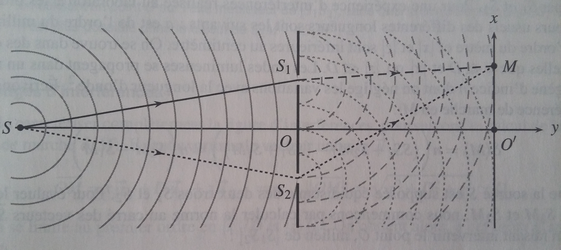
\includegraphics[scale = 0.5]{division.png}
	\end{center}
	\caption{Division du front d'onde par les trous d'Young}
\end{figure}

Cela revient à subordonner les sources secondaires $S_1$ et $S_2$ à une source principale $S$ : le caractère aléatoire de l'émission en $S$ va être masqué, car S1 et S2 vont émettre avec une différence de phase $\Phi$ constante (nulle ou non) dans le temps. Les sources secondaires sont alors cohérentes, ce qui rend possible l'obtention d'interférences visibles.\\

Présenter les miroirs de Fresnel et le biprisme de Fresnel succintement (division du front d'onde seulement). 

\begin{figure}[h!]
	\begin{center}
		\begin{tabular}{cc}
  		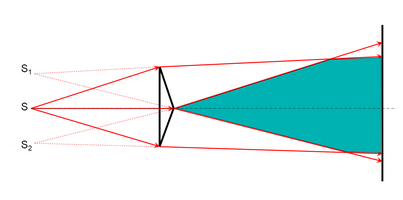
\includegraphics[scale = 0.6]{biprisme.png} &
   		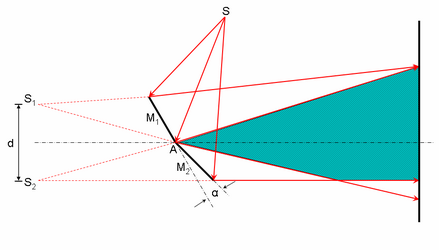
\includegraphics[scale = 0.6]{fresnel_mirrors.png}\\
	\end{tabular}
	\end{center}
	\caption{Champs d'interférences d'un biprisme et des miroirs de Fresnel}
\end{figure}

\newpage
\subsection{Cohérence temporelle}

Puisque les trains d'onde ont une durée $\tau$ finie, ils ne peuvent plus être rigoureusement monochromatiques (l'onde monochromatique ayant une durée infinie, pas de début ni de fin). Si on veut connaître le contenu spectral d'un train d'onde, on calcule sa transformée de Fourier.\\ 

Par exemple, pour un train d'onde d'amplitude constante
\begin{equation}
	s(t) = A\text{cos}\;\left(2\pi\nu_m t\right) \quad\text{entre les instants}\quad -\tau_c/2
	\quad\text{et}\quad\tau_c/2,
\end{equation}

\begin{figure}[h!]
	\begin{center}
		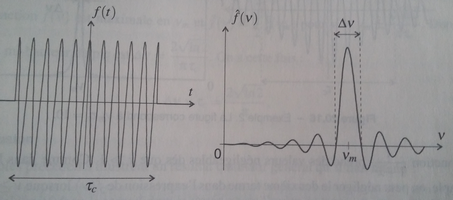
\includegraphics[scale = 0.5]{trainrectangulaire.png}
	\end{center}
	\caption{Train d'ondes rectangulaire de durée $\tau_c$}
\end{figure}

\textbf{Le spectre d'une telle onde n'est évidemment pas monochromatique.} On peut le caractériser par une certaine \textbf{largeur spectrale} $\Delta \nu$, ici la largeur du pic central de ce sinus cardinal.\\

Il existe des modèles plus réalistes pour décrire le spectre d'une source lumineuse : on peut utiliser un profil \textbf{gaussien} (conséquence de l'effet Doppler du fait de l'agitation thermique des atomes émetteurs) ou un profil \textbf{lorentzien} (largeur naturelle de la raie spectrale).\\

\begin{figure}[h!]
	\begin{tabular}{cc}
  		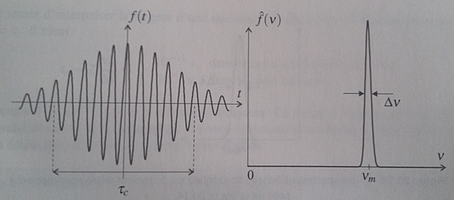
\includegraphics[scale = 0.5]{traingaussien.png} &
   		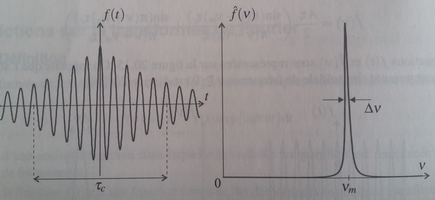
\includegraphics[scale = 0.5]{trainlorentzien.png}\\
	\end{tabular}
	\caption{Trains d'ondes gaussien (gauche) et lorentzien (droite)}
\end{figure}

Une raie spectrale sera caractérisée par sa fréquence moyenne $\nu_m$ et par une certaine largeur spectrale $\Delta\nu$ (que l'on peut aussi exprimer en termes de longueur d'onde $\Delta \lambda$ ou de vecteur d'onde $\Delta k$). On voit que la durée moyenne d'un train d'onde (\textbf{temps de cohérence de la source}) est inversement proportionnelle à la largeur spectrale de la source $\Delta\nu$ :\\
\begin{equation}
	\boxed{\tau_c \sim \frac{1}{\Delta\nu}},
\end{equation}
d'où la \textbf{longueur de cohérence temporelle}
\begin{equation}
	L_c \equiv c\tau_c \sim \frac{c}{\Delta\nu}
\end{equation}
qui correspond à la longueur moyenne des trains d'onde, comme nous l'avons déjà mentionné plus haut.

\subsubsection{Interférences avec deux sources identiques non-monochromatiques}

Nous avons vu que deux ondes de fréquences différentes n'interféraient pas. On peut décomposer le spectre d'une source polychromatique en une superposition de sources monochromatiques et, si on prend deux sources identiques, on obtiendra un \textbf{éclairement égal à la somme des éclairements monochromatiques}. Les figures d'interférence propres à chaque fréquence vont se superposer, "couleur par couleur" induisant un brouillage des franges, \textbf{une perte de contraste}.\\ 

%Pour mettre ce phénomène en évidence, prenons l'exemple de deux sources ponctuelles identiques dont le spectre est constitué de deux raies, que l'on supposera parfaitement monochromatiques (infiniment fines dans l'espace de Fourier) :
%\begin{equation}
%	\lambda_{01} > \lambda_{02} \quad\text{et}\quad \Delta\lambda = \lambda_{01} - \lambda_{02} \ll
%	\lambda_{01,2}.
%\end{equation}
%Ce modèle de spectre convient bien pour décrire le doublet jaune d'une lampe spectrale à vapeur de sodium, $\lambda_{01} = 5895.924\times 10^{-10}$m et $\lambda_{02} = 5889.950\times 10^{-10}$m.\\
%
%L'éclairement total en un point M de l'écran (on se ramène au modèle de la section précédente en ne relâchant que la seule hypothèse des sources monochromatiques), s'écrit
%\begin{equation}
%	\boxed{\mathcal{E}(M) = \underbrace{\mathcal{E}_1(M)}_{\text{radiation}\;\lambda_{0,1}} 
%	+ \underbrace{\mathcal{E}_2(M)}_{\text{radiation}\;\lambda_{0,2}}},
%\end{equation}
%avec
%\begin{equation}
%	\mathcal{E}_i(M) = 2\mathcal{E}_0\left[1 
%	+ \text{cos}\;\left(k_{0i}\delta\right)\right],\quad\text{avec}\quad k_{0,i} 
%	= \frac{2\pi}{\lambda_{0,i}}
%\end{equation}
%
%En utilisant 
%\begin{equation}
%	\text{cos}\;\alpha + \text{cos}\;\beta = 
%	2\text{cos}\left(\frac{\alpha+\beta}{2}\right) 
%	\text{cos}\left(\frac{\alpha-\beta}{2}\right),
%\end{equation}
%on trouve
%\begin{equation}
%	\mathcal{E}(M) = 4\mathcal{E}_0\left[1 
%	+ \text{cos}\;\left(\frac{k_{0,1}-k_{0,2}}{2}\delta\right)
%	\text{cos}\;\left(\frac{k_{0,1}+k_{0,2}}{2}\delta\right)\right],
%\end{equation}
%puis
%\begin{equation}
%	\boxed{\mathcal{E}(M) = 4\mathcal{E}_0\left[1 
%	+ \text{cos}\;\left(\frac{\Delta k_0}{2}\delta\right)
%	\text{cos}\;\left(k_{0m}\delta\right)\right]}.
%\end{equation}
%
%Imaginons que les deux sources en question soient les trous d'Young, comme dans la section précédente, et que l'on observe la figure d'interférences dans un plan perpendiculaire au plan médiateur des sources. Dans ce cas $\delta = ax/D$, $a$ étant l'écart entre les deux trous et $D$ la distance d'observation.\\
%
%Comme $\Delta k_0 \ll k_m$, le second cosinus va varier beaucoup plus rapidement que le premier.

On définit la densité spectrale d'intensité d'une source comme la fonction $g(k)$ telle que
\begin{equation}
	d\mathcal{I}_0 = g(\nu)d\nu
\end{equation}
où $d\mathcal{I}_0$ est l'intensité émise par la source sur une gamme de fréquences comprises entre $\nu$ et $\nu + d\nu$ (et de vecteur d'onde compris entre $k$ et $k+dk$ puisque $2\pi \nu = ck$. Supposons que cette fonction a un profil rectangulaire, de largeur $\Delta k$ entre $k_{0,1}$ et $k_{0,2}$ et d'amplitude constante $\mathcal{I}_0/\Delta k$ \textcolor{red}{(schéma)}. Il s'agît d'une modélisation simplifiée d'une source de faible largeur spectrale, si on suppose  $\Delta k = k_{0,2} - k_{0,1} \ll k_{01,2}$\\

Loin des sources, intensité et éclairement sont proportionnels (l'onde sphérique émise par une source pouvant être considérée, avec une bonne approximation comme une onde plane, en tout cas localement, à l'échelle de l'écran). On somme les éclairements pour obtenir l'éclairement total en un point d'observation M :
\begin{equation}
	\mathcal{E}(M) = \int_{k_{0,1}}^{k_{0,2}} 2d\mathcal{E}_0\left[1 + \text{cos}\;(k\delta(M))\right]
	=  \int_{k_{0,1}}^{k_{0,2}} 2 dk \frac{\mathcal{E}_0}{\Delta k}
	\left[1 + \text{cos}\;(k\delta(M))\right],
\end{equation}
d'où
\begin{equation}
	\boxed{\mathcal{E}(M) = 2\mathcal{E}_0\left[1 + \text{sinc}\;\left(\frac{\Delta k_0}{2}
	\delta\right)\text{cos}\left(k_{0m}\delta(M)\right)\right] 
	= 2\mathcal{E}_0 \left[1 + \gamma(M)\text{cos}\left(k_{0m}\delta(M)\right) \right]},
\end{equation}
où
\begin{equation}
	k_{0m} = \frac{k_{0,1}+k_{0,2}}{2}\quad\text{et}\quad \Delta k_0 = k_{0,2} - k_{0,1}.
\end{equation}
en utilisation le formulaire de trigonométrie.\\

On a introduit $\gamma(M)$ fonction appelée \textbf{degré de cohérence temporelle}. Cette fonction varie beaucoup plus lentement que le terme en cosinus qu'elle va par conséquent moduler en amplitude. On définit la \textbf{visibilité} comme
\begin{equation}
	V(M) = |\gamma(M)|.
\end{equation}

\begin{figure}[h!]
	\begin{center}
		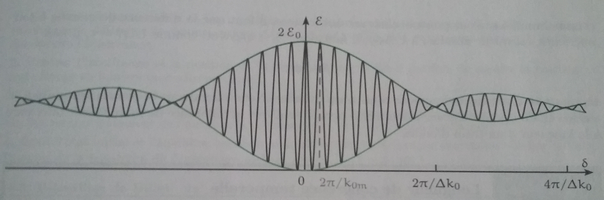
\includegraphics[scale = 0.6]{sourcenonmono.png}
	\end{center}
	\caption{Perte de contraste lié au caractère non-monochromatique d'une source}
\end{figure}

On constate que pour une différence de marche $\delta$ proche de 0, les franges sont bien visibles alors que pour $\delta$ plus importante, on perd en visibilité. On remarque une première annulation de contraste lorsque $\delta = 2\pi/\Delta k_0$. L'éclairement diminue fortement pour des chemins optique plus grands. On en déduit que pour observer des interférences avec un bon contraste, les deux ondes doivent satisfaire
\begin{equation}
	\delta \ll \frac{2\pi}{\Delta k_0} = \frac{c}{\Delta\nu} \sim c\tau_c = L_c 
	\quad\text{et donc}\quad\delta \ll L_c
\end{equation}
puisque $\tau_c \sim 1/\Delta \nu$.\\

Notons que cette figure représente l'éclairement en fonction de $\delta$ mais que, dans le cas d'une observation dans un plan perpendiculaire au plan médiateur des sources, elle représente également l'éclairement tel qu'on le percevrait sur l'écran, puisqu'il y a une relation de proportionnalité entre $\delta$ et la coordonnée spatiale parallèle à l'axe des sources. Ce qui est fort, c'est que \textbf{la figure d'interférences nous donne des informations sur la nature de la source}, d'où de possibles applications en spectroscopie.

\section*{Conclusion}

La lampe à vapeur de sodium émet principalement dans le jaune : cette lumière est constituée en réalité de deux raies spectrales très proches l'une de l'autre, centrées sur
\begin{equation}
	\lambda_{01} = 5895.924\times 10^{-10} m \quad\text{et}\quad 
	\lambda_{02} = 5889.950\times 10^{-10} m,
\end{equation}
avec $\lambda_{01} > \lambda_{02}$ et $\Delta\lambda = \lambda_{01}-\lambda_{02}\ll\lambda_{01,2}$. On caractérise cette source par un écart de fréquences tel que
\begin{equation}
	\frac{\Delta \nu}{\nu} = \frac{\Delta \lambda}{\lambda}.
\end{equation}

Un calcul de même nature que le précédent, en considérant deux raies monochromatiques séparées de $\Delta\nu$, conduit à une longueur de cohérence temporelle
\begin{equation}
	L_c \simeq 6\times 10^{-4} m.
\end{equation}
En utilisant des trous d'Young séparés de 0.1 mm et en observant la figure d'interférences à 2m, on obtiendrait la première annulation de contraste en 
\begin{equation}
	x = \frac{L_c D}{a} = 12 \text{m},
\end{equation}
ce qui est tout bonnement impensable, faute de luminosité. On pourrait éloigner les sources secondaires l'une de l'autre, mais on augmenterait alors la différence de chemin optique $\delta$, qui se rapprocherait dangereusement de la longueur de cohérence, impliquant une perte de contraste. On pourrait songer à ouvrir davantage le trou/fente source pour laisser entrer davantage de lumière, mais comme nous le verrons dans une prochaine leçon, et comme nous l'avons remarqué en introduction, cela résultera en une diminution supplémentaire de la visibilité des franges, du fait d'un défaut de \textbf{cohérence spatiale}.\\

Une source "large" peut en effet être vue comme constituée d'un ensemble de sources ponctuelles incohérentes entre elles, réparties sur une surface ou dans un volume. Ces sources étant incohérentes entre elles, les éclairements de chaque source ponctuelle composant la source étendue vont se superposer et se brouiller. Si la source est suffisamment "peu étendue" par rapport à la taille de l'interféromètre (typiquement la distance entre les deux sources secondaires), on pourra observer des interférences mais avec un contraste affaibli. On définira une longueur de cohérence spatiale $L_s$ comme la largeur maximale de la source donnant une figure d'interférences peu brouillée avec un interféromètre donné. Ceci implique des contraintes assez lourdes, on doit toujours \textbf{rechercher un compromis entre contraste et luminosité}.\\ 

L'interférométrie à division d'amplitude est une technique d'interférométrie différente de celle à division du front d'ondes, permettant de visualiser des interférences en utilisant des sources larges, sans perte de contraste du fait de problèmes de cohérence spatiale. Elle fera l'objet d'une leçon ultérieure.

\newpage
\section*{Annexes}
\subsection*{Manipulation qualitative d'introduction}

Fentes d'Young en lumière spectrale : lampe à vapeur de sodium ou de mercure, avec un filtre approprié.\\

\textbf{Protocole :}
\begin{itemize}
	\item Placer la lampe et un écran, à environ deux mètres de là où seront placées les bifentes.
	\item Placer les bifentes et un condenseur, former l'image de la lampe sur les bifentes pour faire passer un maximum de lumière et commenter : on voit un gros pâté.
	\item Placer une fente source de largeur réglable juste après le condenseur. Commenter en réduisant progressivement la largeur de la fente source jusqu'à apparition de franges d'interférences. Bizarre bizarre.
\end{itemize}
\end{document}